\documentclass{standalone}
\usepackage{tikz}
\usepackage{xcolor}
\usetikzlibrary{patterns, positioning}
\usetikzlibrary{shapes.misc}
\usepackage[outline]{contour}
\contourlength{1.5pt} 


\begin{document}
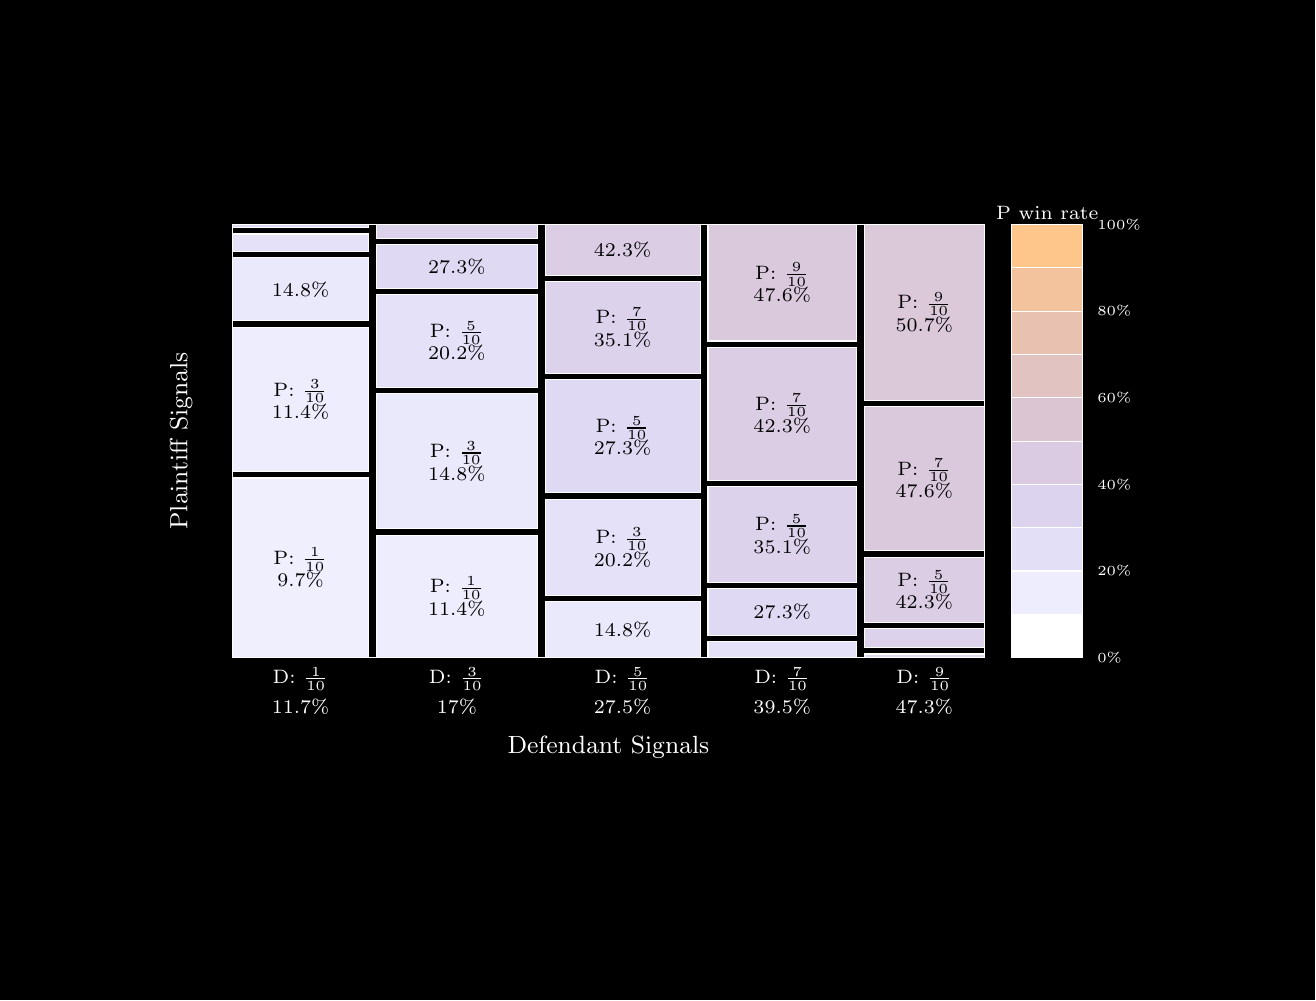
\begin{tikzpicture}
\newcommand{\DFractionOffset}{0.4}
\newcommand{\AxisLabelYAdjust}{-0.235}
\pagecolor{black}
\draw[fill=black, draw=none] (-2,-2) rectangle (14,10);
\draw[draw=white] (0.6,2) rectangle (10.15,7.5);
\draw[fill=blue!90!orange!10!white!68!white, draw=white] (0.6,2) rectangle (2.3306,4.2811);
\draw (1.465318179857591, 3.1405278113665935) node[font=\scriptsize, text=black, align=center] {P: $\frac{1}{10}$\\ 9.7\%};
\draw[fill=blue!89!orange!11!white!67!white, draw=white] (0.6,4.3611) rectangle (2.3306,6.1956);
\draw (1.465318179857591, 5.27830420309013) node[font=\scriptsize, text=black, align=center] {P: $\frac{3}{10}$\\ 11.4\%};
\draw[fill=blue!85!orange!15!white!66!white, draw=white] (0.6,6.2756) rectangle (2.3306,7.0795);
\draw (1.465318179857591, 6.677528776159923) node[font=\scriptsize, text=black, align=center] {14.8\%};
\draw[fill=blue!80!orange!20!white!65!white, draw=white] (0.6,7.1595) rectangle (2.3306,7.3794);
\draw[fill=blue!73!orange!27!white!63!white, draw=white] (0.6,7.4594) rectangle (2.3306,7.5);
\draw (1.465318179857591, 1.6) node[anchor=north, font=\scriptsize, text=white] {11.7\%};
\draw (1.465318179857591, {1.6 + \DFractionOffset}) node[anchor=north, font=\scriptsize, text=white] {D: $\frac{1}{10}$};
\draw[fill=blue!89!orange!11!white!67!white, draw=white] (2.4306,2) rectangle (4.4714,3.5557);
\draw (3.4510408711637344, 2.7778404183108583) node[font=\scriptsize, text=black, align=center] {P: $\frac{1}{10}$\\ 11.4\%};
\draw[fill=blue!85!orange!15!white!66!white, draw=white] (2.4306,3.6357) rectangle (4.4714,5.3499);
\draw (3.4510408711637344, 4.492773260341328) node[font=\scriptsize, text=black, align=center] {P: $\frac{3}{10}$\\ 14.8\%};
\draw[fill=blue!80!orange!20!white!65!white, draw=white] (2.4306,5.4299) rectangle (4.4714,6.611);
\draw (3.4510408711637344, 6.020454310291027) node[font=\scriptsize, text=black, align=center] {P: $\frac{5}{10}$\\ 20.2\%};
\draw[fill=blue!73!orange!27!white!63!white, draw=white] (2.4306,6.691) rectangle (4.4714,7.2425);
\draw (3.4510408711637344, 6.966752888653639) node[font=\scriptsize, text=black, align=center] {27.3\%};
\draw[fill=blue!65!orange!35!white!61!white, draw=white] (2.4306,7.3225) rectangle (4.4714,7.5);
\draw (3.4510408711637344, 1.6) node[anchor=north, font=\scriptsize, text=white] {17\%};
\draw (3.4510408711637344, {1.6 + \DFractionOffset}) node[anchor=north, font=\scriptsize, text=white] {D: $\frac{3}{10}$};
\draw[fill=blue!85!orange!15!white!66!white, draw=white] (4.5714,2) rectangle (6.5394,2.707);
\draw (5.555402771968875, 2.353508330872114) node[font=\scriptsize, text=black, align=center] {14.8\%};
\draw[fill=blue!80!orange!20!white!65!white, draw=white] (4.5714,2.787) rectangle (6.5394,4.0119);
\draw (5.555402771968875, 3.3994814952157775) node[font=\scriptsize, text=black, align=center] {P: $\frac{3}{10}$\\ 20.2\%};
\draw[fill=blue!73!orange!27!white!63!white, draw=white] (4.5714,4.0919) rectangle (6.5394,5.5301);
\draw (5.555402771968875, 4.811030286495934) node[font=\scriptsize, text=black, align=center] {P: $\frac{5}{10}$\\ 27.3\%};
\draw[fill=blue!65!orange!35!white!61!white, draw=white] (4.5714,5.6101) rectangle (6.5394,6.7764);
\draw (5.555402771968875, 6.193272657040394) node[font=\scriptsize, text=black, align=center] {P: $\frac{7}{10}$\\ 35.1\%};
\draw[fill=blue!58!orange!42!white!59!white, draw=white] (4.5714,6.8564) rectangle (6.5394,7.5);
\draw (5.555402771968875, 7.178215534888123) node[font=\scriptsize, text=black, align=center] {42.3\%};
\draw (5.555402771968875, 1.6) node[anchor=north, font=\scriptsize, text=white] {27.5\%};
\draw (5.555402771968875, {1.6 + \DFractionOffset}) node[anchor=north, font=\scriptsize, text=white] {D: $\frac{5}{10}$};
\draw[fill=blue!80!orange!20!white!65!white, draw=white] (6.6394,2) rectangle (8.527,2.2016);
\draw[fill=blue!73!orange!27!white!63!white, draw=white] (6.6394,2.2816) rectangle (8.527,2.8778);
\draw (7.583155146943383, 2.57967632467773) node[font=\scriptsize, text=black, align=center] {27.3\%};
\draw[fill=blue!65!orange!35!white!61!white, draw=white] (6.6394,2.9578) rectangle (8.527,4.1737);
\draw (7.583155146943383, 3.5657403761033915) node[font=\scriptsize, text=black, align=center] {P: $\frac{5}{10}$\\ 35.1\%};
\draw[fill=blue!58!orange!42!white!59!white, draw=white] (6.6394,4.2537) rectangle (8.527,5.9407);
\draw (7.583155146943383, 5.097217297062647) node[font=\scriptsize, text=black, align=center] {P: $\frac{7}{10}$\\ 42.3\%};
\draw[fill=blue!52!orange!48!white!58!white, draw=white] (6.6394,6.0207) rectangle (8.527,7.5);
\draw (7.583155146943383, 6.760359994160356) node[font=\scriptsize, text=black, align=center] {P: $\frac{9}{10}$\\ 47.6\%};
\draw (7.583155146943383, 1.6) node[anchor=north, font=\scriptsize, text=white] {39.5\%};
\draw (7.583155146943383, {1.6 + \DFractionOffset}) node[anchor=north, font=\scriptsize, text=white] {D: $\frac{7}{10}$};
\draw[fill=blue!73!orange!27!white!63!white, draw=white] (8.627,2) rectangle (10.15,2.0462);
\draw[fill=blue!65!orange!35!white!61!white, draw=white] (8.627,2.1262) rectangle (10.15,2.3641);
\draw[fill=blue!58!orange!42!white!59!white, draw=white] (8.627,2.4441) rectangle (10.15,3.2756);
\draw (9.388475066280652, 2.859828496016138) node[font=\scriptsize, text=black, align=center] {P: $\frac{5}{10}$\\ 42.3\%};
\draw[fill=blue!52!orange!48!white!58!white, draw=white] (8.627,3.3556) rectangle (10.15,5.1889);
\draw (9.388475066280652, 4.272274337211412) node[font=\scriptsize, text=black, align=center] {P: $\frac{7}{10}$\\ 47.6\%};
\draw[fill=blue!49!orange!51!white!57!white, draw=white] (8.627,5.2689) rectangle (10.15,7.5);
\draw (9.388475066280652, 6.384473132251992) node[font=\scriptsize, text=black, align=center] {P: $\frac{9}{10}$\\ 50.7\%};
\draw (9.388475066280652, 1.6) node[anchor=north, font=\scriptsize, text=white] {47.3\%};
\draw (9.388475066280652, {1.6 + \DFractionOffset}) node[anchor=north, font=\scriptsize, text=white] {D: $\frac{9}{10}$};
\node[font=\small, text=white] at (5.375, {1.1 + \AxisLabelYAdjust}) {Defendant Signals};
\node[font=\small, text=white, rotate=90] at (-0.050000000000000044, 4.75) {Plaintiff Signals};
\draw[draw=white] (10.5,2) rectangle (11.4,7.5);
\draw (10.95, 7.65) node[font=\scriptsize, text=white] {P win rate};
\draw[fill=blue!100!orange!0!white!70!white, draw=white] (10.5,2) rectangle (11.4,2.55);
\draw[fill=blue!89!orange!11!white!67!white, draw=white] (10.5,2.55) rectangle (11.4,3.1);
\draw[fill=blue!78!orange!22!white!64!white, draw=white] (10.5,3.1) rectangle (11.4,3.65);
\draw[fill=blue!67!orange!33!white!62!white, draw=white] (10.5,3.65) rectangle (11.4,4.2);
\draw[fill=blue!56!orange!44!white!59!white, draw=white] (10.5,4.2) rectangle (11.4,4.75);
\draw[fill=blue!44!orange!56!white!56!white, draw=white] (10.5,4.75) rectangle (11.4,5.3);
\draw[fill=blue!33!orange!67!white!53!white, draw=white] (10.5,5.3) rectangle (11.4,5.85);
\draw[fill=blue!22!orange!78!white!51!white, draw=white] (10.5,5.85) rectangle (11.4,6.4);
\draw[fill=blue!11!orange!89!white!48!white, draw=white] (10.5,6.4) rectangle (11.4,6.95);
\draw[fill=blue!0!orange!100!white!45!white, draw=white] (10.5,6.95) rectangle (11.4,7.5);
\draw (11.46, 2) node[anchor=west, font=\tiny, text=white] {0\%};
\draw (11.46, 3.1) node[anchor=west, font=\tiny, text=white] {20\%};
\draw (11.46, 4.2) node[anchor=west, font=\tiny, text=white] {40\%};
\draw (11.46, 5.3) node[anchor=west, font=\tiny, text=white] {60\%};
\draw (11.46, 6.4) node[anchor=west, font=\tiny, text=white] {80\%};
\draw (11.46, 7.5) node[anchor=west, font=\tiny, text=white] {100\%};


\end{tikzpicture}
\end{document}